\chapter{Is market power in Australia growing?\label{chap:trends}}

There is considerable concern in Australia that concentration is rising. Some believe that mergers and acquisitions are concentrating market power in just a handful of large firms. Others believe that the largest firms are growing faster than their smaller competitors, or that smaller competitors are finding it less viable to challenge industry incumbents.%
    \footcites{Janda_merger_2008}{IBISWorld_Bunnings_2015}{Bouris_BigBusiness_2015}

Regulators and politicians appear to believe market concentration in Australia has increased.

\begin{quote}
    `The rise of large corporations in the Australian economy has been substantial. Indeed it seems we have outpaced the US.'
    
    \rightline{-- Rod \textcite{Sims-2016-Keynote-RBB-Concentration}, ACCC Chair}
\end{quote}

\begin{quote}
    `[There seems to be a] general trend [to greater concentration, and] it seems likely that [it has] played a part in the steady rise in inequality.'
    
    \rightline{-- Andrew \textcite{Leigh-2016-Markets&Monopolies}, Shadow Assistant Federal Treasurer}
\end{quote}

% \begin{quote}
%     `Big business has grown at the expense of the public sector through privatisation and at the expense of independent small businesses through increased market concentration.'
    
%     \rightline{-- John \textcite{Quiggin_socialism}, Professor of Economics, University of Queensland}
% \end{quote}

% Evidence is clear in the US that revenue shares of the top four firms have risen in most industries in the past two decades. Some part of this is due to natural growth of productive and globally competitive firms, such as Google (Alphabet) and Apple. But also some part is due to mergers increasing concentration within industries, such as in banking.

% However, \Chapref{chap:international} showed that the US was not a good comparison to Australia due to its size and unusually unconcentrated economy in many sectors at the national level. Some of the rising concentration in the US is firm expansion into new states (for example Walmart%http://metrocosmblog.tumblr.com/post/165807691953/how-walmart-took-over-the-us
% ) where they had no previous presence. Or part of a long process of consolidating highly fragmented industries, such as banking. %http://www.motherjones.com/politics/2010/01/bank-merger-history/

% As a growing economy, there may be room for more firms in each industry than there was 20 years ago. But technology has increased economies of scale for large firms. This could make it harder for small, new entrants to gain market share and grow to a minimum efficient size. However, increasing levels of concentration could signal weaker competitive pressure, which would have adverse impacts on consumers and the economy. 
% %Competitive pressure changes in industries as technology, regulations and market size change. This manifests as increasing or decreasing concentration within industries. If concentration is increasing it could be a sign that large firms are gaining market power, which can be bad for consumers. But is concentration worse than it used to be?

But there is no evidence that competitive pressure in Australia has systematically deteriorated. 

Australia's largest firms have held a steady revenue-share of the economy for more than 20 years. Over the past 20 years the average profitability of firms, and of highly profitable firms, has not changed much.

And there is not much to suggest that major concentrated markets have become more concentrated, on average. A few major sectors have become more concentrated, including banks and (earlier in the 2000s) insurers. Some major sectors have become less concentrated, such as supermarkets and fuel retailing, though they both remain highly concentrated, and the major supermarkets are now also major fuel retailers. 
\section{The biggest listed firms in the non-traded sector are not a larger share of the ASX or the economy}

\doublecolumnfigure{
    \caption{Revenues of large listed firms have not grown faster than revenues of smaller firms\label{fig:ShareASX}}
    \units{Percentage of all revenue reported by ASX-listed firms}
    \includegraphics[page=11]{atlas/Charts}
    \noteswithsource{Top firms are the largest by reported revenue for each year. Excludes Exchange-Traded Funds (ETFs), foreign-headquartered firms, and mining and metals. Includes firms producing tradeables. Nominal values across financial years.}{Grattan analysis of \textcite{Morningstar2017}.}
}%
{
    \caption{Revenues of large listed firms have not grown faster than GDP \label{fig:Top50GDP}}
    \units{Ratio of top 100 listed firms' revenue to GDP, per cent}
  \includegraphics[page=12]{atlas/Charts} 
  \noteswithsource{Top 100 firms by market capitalisation with positive revenue. Non-mining firms is 100 firms excluding Metals and Mining. Non-mining, excluding Woolworths, Telstra and AMP is 100 firms excluding these three large ASX listings. Most of the early increase is due to the relisting of Woolworths in 1993, and the listing of AMP and Telstra later in the 1990s. Excludes Exchange-Traded Funds (ETFs) and foreign-headquartered firms. Includes firms producing tradeables.  }{Grattan analysis of \textcites{Morningstar2017}{ABS2016SystemNationalAccounts}.}
}

The fortunes of individual listed firms wax and wane over the years, but the revenue of large ASX-listed firms has not grown faster than the revenue of smaller listed firms (\Vref{fig:ShareASX}).

% There is no discernible trend in revenue shares of the largest 20, 50, 100 and 200 firms is compared to all ASX revenues, as shown in \Vref{fig:ShareASX}. This indicates that within the ASX there has been no concentration of revenue to a few large firms due either to mergers or natural firm growth. The largest public firms in Australia tend to be banks, supermarkets and miners, but their share relative to the rest of the ASX and compared to GDP has been steady.

Neither has the revenue of Australia's largest non-mining firms changed much compared to GDP, as seen in \Vref{fig:Top50GDP}. Combined, the revenues of the largest 100 publicly traded Australian firms outside the mining sector have equalled about 30-to-40 per cent of GDP since 1994.%
    \footnote{The observation of ACCC Chair Rod Sims cited above (\textcite{Sims-2016-Keynote-RBB-Concentration}) relied on analysis that appears to have included only firms that were still listed on the ASX at the end of the time period examined, and to have excluded firms that delisted in years prior, leading to an incorrect finding that the revenues of the largest ASX-listed firms have grown faster than GDP over time.}

%\hl{However, SOURCE X, which includes both listed and listed firms, suggests that the size distribution of firms has not changed much between XXXX and XXXX.}

%This indicates the ASX is not becoming more, or less, representative of all Australian businesses.

In contrast, in the US the revenue of the Fortune 100 has risen relative to GDP and to the Fortune 500. Mergers and acquisitions, and organic growth (for example, the emergence of large tech firms such as Facebook, Amazon, Google and Apple), have both played a role.%
    \footcite{Econsuperstar2016}


\section{Competitive pressure in many large, concentrated sectors has not waned}

Competitive pressure within large, concentrated sectors appears to have changed little over the past 10 years, although publicly available data is too limited to analyse every sector in the non-traded private economy.

% \begin{figure}
%     \caption{Average industry concentration has not moved much since 2001 \label{fig:ASX-HHI}}
%     \units{Industry revenue weighted concentration index of ASX listed Australian, non-mining firms, 1993 to 2016, 1993 = 100}
%     \includegraphics[page=3]{atlas/ChartsLucy}
%     \noteswithsource{A number of large firms listed on the ASX around 1999 including Telstra and AMP which cause a short term rise in concentration on the ASX\@. Concentration index calculated using the Herfindahl index, weighted by industry revenue. Excludes Exchange Traded Funds (ETFs), foreign headquartered firms and mining and metals. Includes firms producing tradables. Nominal values across financial years.}{Grattan analysis of \textcite{Morningstar2017}.}
% \end{figure}

% Total firm numbers have increased within most board ANZSIC industry groupings since 2007. Although there have been short periods over which firms numbers have declined, there has been no long-term trend of net-firm decline.%
% \footnote{ref: Andrew Leigh
% % http://www.andrewleigh.com/markets_monopolies_moguls_speech
% .}

% Aggregate industry concentration of publicly-listed firms is around the same level today as it was 15 years ago. \Vref{fig:ASX-HHI} shows a revenue-weighted aggregate measure of intra-industry concentration for Australian ASX-listed firms.  This measure excludes foreign and privately owned firms, and many Australian firms now face competition from these firms. Supermarkets are subject to increasing competition from Aldi and Costco, Telstra competes with Singaporean Optus, and Australian news and media firms compete with international firms online. %
% \footnote{This is not a complete measure of economy wide concentration as not all firms are publicly listed, but the largest firms tend to be publicly listed. In banking, ICT infrastructure, and supermarkets, which are large, highly concentrated industries, the largest firms are publicly listed.}

Concentration in the largest sectors with barriers to entry has not changed much on average. Large banks acquired smaller firms, and their market shares rose as a result. The largest firms in mobile telecommunications, supermarkets, reinsurance, and retail and wholesale fuel have lost market share (\Cref{fig:mobile-supermarket-banking} and \Vref{fig:insurance-fuel}).

Some smaller sectors become more concentrated, including meat processing, breweries and soft drinks.\footcite{Leigh-2016-Markets&Monopolies} One study found preliminary evidence that concentration rose across the whole economy between 2003 and 2015. But the study is difficult to interpret because the sector groups are quite large and it did not identify which sectors became more concentrated, give more weight to larger sectors, or separate non-tradeables and tradeables.%
  \footcite{Bakhtiari_2017}


\doublecolumnfigure{
    \caption{Concentration has fallen in supermarkets, and risen in banking \label{fig:mobile-supermarket-banking}}
    \units{Market share, per cent}
    \includegraphics[page=13]{atlas/Charts} 
    \noteswithsource{Wireless telcom.: market share defined by mobile phone subscribers, including resellers. Supermarkets: market shared defined by total revenue. Banks: market share defined by gross loans and advances.}{Grattan analysis of \textcites{ACCC2016TelecommunicationsReports}{RoyMorgan2017SingleSource}{APRA2017MonthlyBankingStatistics}.}
}{
    \caption{Concentration has changed little in insurance, and has fallen in petrol retailing \label{fig:insurance-fuel}}
    \units{Market share, per cent}
    \includegraphics[page=14]{atlas/Charts} 
    \noteswithsource{Consolidated insurers: market share defined by gross earned premium (QBE adjusted for foreign-earned premium. Reinsurers: market share defined by gross written premium. Fuel retail and wholesale: market share defined by total revenue.}{Grattan analysis of \textcites{APRA_insurance_2017}{ACCC_Petrol_2014}.}
}

\subsection{Banks}
The market share of the largest two banks increased around the time of the global financial crisis: Westpac acquired St George bank, and Commonwealth Bank acquired Bankwest from its financially distressed parent bank in the UK\@.%
\footnote{\Cref{fig:mobile-supermarket-banking} shows the merger of Commonwealth and Bankwest in 2012, which is when APRA reporting was integrated.}
The major banks have lost a little market share since then. 

\subsection{Supermarkets}

The two large supermarket chains, Coles and Woolworths, have lost market share since 2005. They will probably lose more share. The main recent international entrants, Aldi and Costco, plan to expand further. Amazon Fresh and Kaufland are expected to begin operating in Australia soon.\footcites{Kaufland_2017}{AmazonFresh_2017} %
Consumers are likely to benefit from greater diversity and lower prices.\footnote{As just one example, the two major supermarkets, which tend to be higher priced than Aldi (\textcite{Choice-supermarket-want-to-spend-less}), dropped their prices in response to an Aldi store opening in their vicinity (\textcite{ACCC-grocery-2008}), though more recently they have moved to statewide pricing.}


\subsection{Mobile telecommunications}

Concentration in mobile telecommunications rose in 2009 when Vodafone, the third-largest network, bought Hutchison, the smallest of the four networks, reducing the number of networks to three. The regulator approved the acquisition on the basis that it was likely to result in a stronger third competitor in the market. Vodafone is one of the largest mobile operators globally.\footcite{ACCC_mobile_2009} 

When market share of subscribers is measured to include resellers, the share of the three big networks has fallen. Resellers may not increase price competition in Australia much yet, though they do shop around from network for network. 

Mobile telecommunications is a relatively new sector, and network technology develops fast, so it is difficult to forecast how the market might evolve. For example, new operators using long-range forms of Wi-Fi might become viable competitors for some current uses of mobile networks. And the networks' planned 5G systems might also come to pose strong competition for some fixed-line internet services.

\subsection{Fuel wholesale and retail}

Independent firms have gained market share in fuel retailing markets over the past 10 years.%
\footnote{Independent retailers are retailers (owning single or multiple sites) other than supermarket retailers and refiner-wholesalers, \textcite{ACCC_Petrol_2014}.} They also gained a small share in wholesaling. But both markets remain highly concentrated.%
%, which is common across high-income countries.

The retail petrol industry has changed substantially. Retailers are no longer mostly integrated with refiners. The retail fuel market has become more integrated with supermarkets, an evolution from co-branded service stations accepting shopper-dockets for fuel discounts. At the same time, the market share of independent retailers (including 7-Eleven) has tripled from 6 per cent to 19 per cent.\footcite{ACCC_Petrol_2014}

The wholesale petrol industry has become less dependent on the local refineries since the mid-2000s. Independent wholesalers have increased their import capacity from 3 per cent to 8 per cent.\footcite{ACCC_Petrol_2014}

\subsection{General, life and health insurance}

Some evidence suggests the general, life and health insurance sectors have become more concentrated since the early 2000s. But they have been stable in recent years.%
\footcites{APRA_insurance_2017}{APRA_FSI_2014}

In \textbf{general insurance},  APRA reports there was a period of increasing concentration in the early 2000s after HIH Insurance collapsed.\footnote{Not shown in \Cref{fig:mobile-supermarket-banking} due to lack of available data. \textcite{APRA_FSI_2014}.} Recently, both consolidated direct insurance and reinsurance have had steady concentration levels, as shown in \Vref{fig:mobile-supermarket-banking}. Reinsurers show no trend over the past decade, and consolidated insurers have had stable concentration levels since 2012.%
  \footnote{Consolidated insurer data is not available before 2012.}


In \textbf{life insurance}, the total number of firms licensed to sell life insurance has fallen from 55 in 1992, to 36 in 2002 and 21 in 2012. This is the result of mergers and foreign insurers withdrawing from the Australian market.%
\footnote{A decline in the number of licences may not affect competition if firms with small market shares exit. \textcite{APRA_insight_insurance}.} But concentration measured by assets has been relatively stable for the past decade.%
\footcite{APRA_PC_Sub_2017} 

In \textbf{health insurance}, licence numbers have declined over the past 20 years. There are currently 36 licensed health insurers, in the mid-1990s there were around 50 licensed health insurers.%
\footcites{PHIAC-competition-health}{APRA_PC_Sub_2017} Since 2011 concentration by insurance polices has been relatively stable in the health insurance sector.

Concentration in the insurance sectors increased in part due to the privatisation of government insurers and demutualisation of mutually owned insurers, some of which later merged with other firms.

The insurance industry also became more concentrated due to APRA's prudential framework changes.
Before the collapse of HIH Insurance, `unsustainable competition' had been driving down premium prices and resulting in erratic returns.
  \footcite[][23--24]{APRA_FSI_2014}
In APRA's judgement, the general insurance sector is now a `safer, more efficient and more competitive industry'.%
  \footcite[][23]{APRA_FSI_2014}  


% Australian consumers may be affected by the rising market share of international firms, such Anheuser-Busch InBev, but Australia's home-grown firms are not exhibiting the same trends. Apple, Google and 

% In general insurance, concentration has been relatively stable after a period of industry adjustment in the early 2000s (not shown in \Cref{fig:mobile-supermarket-banking} due to lack of available data).
% Reinsurers show no trend over the past decade, and consolidated insurers have had stable concentration levels since 2012.%
%   \footnote{Consolidated insurer data is not available before 2012.}

\begin{bigbox}{Mergers, acquisitions and market concentration}{box:Mergers}
Some have pointed to the role of mergers and acquisitions (M\&A) in increasing concentration. For example, \textcite{Leigh-Triggs-Huff-2017} remark:

\begin{quote}
    In many industries, Australia's markets are more concentrated than those in comparable countries. We also find some evidence that the problem is getting worse. For example, the number of mergers and acquisitions has nearly tripled since 1992.
\end{quote}  


Some acquisitions in Australia have increased concentration. In banking, concentration increased in 2008 when the Commonwealth Bank acquired Bankwest (though this increased financial stability), and Westpac acquired St George.%
\footcite{APRA2017MonthlyBankingStatistics}
In mobile telecommunications, concentration increased when Vodafone acquired Hutchison (Three), though this may have resulted in a more viable third competitor to the larger two firms in that market. Mergers have also been an important factor in the increasing concentration in the US, where some analysts argue that anti-trust enforcement has been too weak.%
\footcite{antitrustpopulism}

But M\&A activity does not necessarily increase market power.
First, mergers are tightly governed by competition law and must be approved by the ACCC\@. The effects on competition of a proposed merger are considered by the ACCC\@.%
\footcite{ACCC_mergerguidelines}

Second, international acquisitions do not affect Australia's non-traded private economy.
Rio Tinto's merger with Alcan in 2007 had little effect on competition in Australia.

Third, cross-sector acquisitions may not change market power much and may even decrease it. Wesfarmers' acquisition of Coles did not increase supermarket concentration. 7-Eleven's acquisition of Mobil Oil Australia's retail fuel sites decreased fuel retailing concentration.\footcite{7eleven_divestment}

Fourth, M\&A may not increase market concentration in the long term if smaller firms are growing fast enough. Woolworths and Metcash's combined acquisition of parts of Foodland's Australian business in 2005 temporarily boosted concentration, but this was more than offset in subsequent years by Aldi's gain in market share.\footcite{FT_Foodland_2005}

Fifth, in the tradeables sectors, M\&A activity that increases the apparent level of concentration will often not give the enlarged firm more market power. For example, the ACCC found that Xstrata's acquisition of MIM Holdings was `unlikely to substantially lessen competition', in part because Australia's markets for thermal and coking coal are integrated into global markets.%
  \footnote{\textcite{ACCC_Xstrata}. The tradeables sectors are about the same size as the sum of the high-barriers sectors.}

Similarly, transactions in sectors with low barriers to entry do not increase market power much. These sectors are about three times the size of sectors with high barriers to entry. Acquisitions such as Quadrant's acquisitions of Goodlife Health Clubs, Jetts Australia and Fitness First Australia do not reduce competitive intensity much.\footcite{ACCC_Fitness}

For these reasons, the level of aggregate M\&A provides little guidance to whether markets are becoming more concentrated.

% In 2007 merger activity peaked at 3,059 mergers and acquisitions, worth \$US 348 billion. Mergers ad acquisitions have slowed since, now around the same as in the early 2000s. But this is not increasing economy-wide concentration.

% Mergers and acquisitions increase concentration, and market power, if they are not equally offset by firm creation and growth, and subsidiary divestments. High volumes of mergers is insufficient evidence of concentration and market power. As other concentration measures in Australia have not substantially changed, the merger and acquisition level seems to be at a sustainable level which does not increase concentration.

% Mergers and acquisitions tend to be cyclical, moving with high market valuations and broader business trends. Three factors should be considered regarding high merger activity. Firstly, the peak in 2007 coincided with high market valuations prior to the Global Financial Crisis. This makes merger activity appear to be happening among larger firms than is the case. Merger values are not strictly comparable between years. High valuations also stimulate merger activity which is not associated with a secular trend of increasing concentration. Secondly, there is some evidence the 2007 merger and acquisition peak was low compared to previous cycles. Increasing concentration due to merger activity needs to be disaggregated from cyclical merger activity. And thirdly, the 2007 peak in mergers may have been boosted by international acquisitions, such as Rio Tinto's acquisition of Alcan, a Canadian firm. Mergers and acquisitions across boarders and in tradable sectors do not decrease competitive pressure in the non-traded private sectors.%
%     \footnote{Merger activity is very cyclical, the recent 2007 peak was low relative to historical merger activity. ref: \url{http://vuir.vu.edu.au/15969/1/Socrates_Karagiannidis.pdf} and \url{https://imaa-institute.org/mergers-and-acquisitions-statistics/}.}
    
% The available data for mergers and acquisitions is limited, and individual sector analysis is not possible. But the available evidence indicates that merger activity is not high enough to change economy-wide concentration. 
\end{bigbox}



\section{Firm profitability has been steady since the mid-1990s}

\begin{figure}
    \caption{Profitability has not changed much \label{fig:ASXROEspreads}}
    \units{Percentage of shareholder equity, top 200 listed firms by market capitalisation}
  \includegraphics[page=15]{atlas/Charts} 
  \noteswithsource{Top 200 is excluding Exchange-Traded Funds (ETFs), foreign-headquartered firms, mining and metals, and firms with negative equity. Includes firms producing tradeables. Financial years.}{Grattan analysis of \textcite{Morningstar2017}.}
\end{figure}

Another measure of competitive intensity is profit. The average return on equity of large listed Australian firms has been steady since the mid-1990s. Between 1995 and 2001, the equity-weighted average return on equity of the top-200 ASX firms was 11.8 per cent. Between 2002 and 2008, the equity-weighted average returns rose to 12.7 per cent. Recently, between 2009 and 2015, the equity-weighted average returns of the top-200 ASX firms has fallen to 11.1 per cent (\Vref{fig:ASXROEspreads}).\footnote{Excludes metals and mining, foreign firms, exchange-traded funds and firms with negative equity (\textcite{Morningstar2017}).}

% Profitability has fallen back from its peak in 2006 but has remained consistently above the levels of 1995 to 2002.
% The gap between the most and least profitable firms also grew . Changes in market concentration in Australia have probably been too small to have contributed much to the change in profitability. 

The US has experienced a widening spread of firm returns over the same period.\footnote{\textcite{Econtoohigh2016} The increasing spread of returns may not persist if returns are weighted by invested capital, or equity.} 
In the US, some analysts have suggested that rising market concentration played an important role.%
    \footcites{CEAcompetitionbriefmay2016}{Ganapati_concen_2017}


The small increase in the spread of profitability in the mid-2000s is likely to be due to other factors, such as the generally buoyant conditions, and a decline in the costs of debt in more recent years. The rise of `superstar firms' may also have played a role. Superstar firms earn high returns thanks to differentiated intellectual property, or strong network effects.%
    \footcites{UNCTAD_2017}{AutorDorn2017}
The growth of such sectors (which include pharmaceuticals and internet platforms) is a key contributor to the rising spread of profitability in the US.%
    \footcite[][71--76]{Koller_ROIC_2010}
In turn the rise of these sectors reflect shifts in demand and technology, as well as protections for intellectual property.%
    \footnote{Larger firms do not have higher returns. Firm revenue size is not associated with higher return on invested capital (ROIC), but higher revenue growth is associated with higher ROIC. \textcite{Koller_ROIC_2010}.}

In Australia, such sectors are not as large as in the US, but they are big enough to make a difference to the overall spread of returns. For example, in 2015 about half of the most profitable top-200 ASX firms were technology, platform, or otherwise innovative firms.%
    \footnote{Ranked by return on equity, 11 of the top 20 were firms in software, internet services, biotechnology, medical technology, professional services or IP services. These firms were: IPH Limited, Altium Limited, OFX Group Limited, CSL Limited, Carsales.com Limited, Cochlear Limited, REA Group Ltd, Speedcast International Limited, Technology One Limited, Monadelphous Group Limited, and Sirtex Medical Limited (\textcite{Morningstar2017}).}
While these firms  have pricing power, in many cases it is better thought of as a return to innovation or to intellectual property than to a dominant share of a broader market.%
%\footnote{Competition olicy issues in more technology-driven sectors include the duration and type of intellectual property provision, or on reducing entry costs or customer switching costs. \Chapref{chap:policy} considers these issues.}

\section{Other measures of competitive pressure}

Other metrics, such as net firm creation and investment, are often used as indicators of competitive pressure and business dynamism.%
\footcites{CEAcompetitionbriefmay2016}{Leigh-triggs-AER}

\subsection{Firm dynamism}

\begin{figureTop}
    \caption{One measure of firm ‘dynamism’ has slowed\label{fig:dynamism}}
    \units{Firm creation and destruction as a percentage of incumbent firms} \vspace{3pt} 
    \includegraphics[page=3]{atlas/ChartsLucy_stunted}\vspace{5pt}
    
    \units{Net firms created, thousands}
    \includegraphics[page=4]{atlas/ChartsLucy_stunted} 
    \source{\textcite{ABS-2017-Count-of-Australian-businesses}.}
\end{figureTop}

Firm creation has slowed in Australia since at least the mid-2000s (\Vref{fig:dynamism}); in the US there has been a longer-run decline.%
\footcites{CEAcompetitionbriefmay2016, Furman_preso_2016} 
Some regard firm creation as a measure of dynamism and competitive pressure. It may also be important to employment growth, because young, fast-growing firms are responsible for most employment growth.\footcite{Industry_2015}

The decline in firm creation may not be a problem. The firm exit rate has also declined overall (according to ABS data shown in \Cref{fig:dynamism}), largely offsetting the fall in firm entry.%
    \footnote{\textcites{Breunig_2007}{IllusionsEntrepreneur2010}.
The exit rate of younger firms may have spiked temporarily around 2011, though the causes are not well understood (\textcite{Bakhtiari_2017}).}
In any event, there is not much reason to think the decline in firm creation rates is due to any increase in the market power of large firms. 

%However, if potential new businesses which bring new technologies to the market are deterred by big incumbent firms, productivity growth would be slower. But large firms tend to have economies of scale, making them more efficient than small firms within an industry. Given Australia has a large number of small firms, it is possible that high net firm creation could make Australian industries less efficient and less internationally competitive.
    %http://www.rba.gov.au/publications/confs/2015/andrews-criscuolo-gal-menon.html

\subsection{Investment}

Similarly, non-mining investment in Australia is low by historic standards. Some commentators have suggested that incumbent oligopolists might not invest much.%
    \footcite{Econ_probprofits2016} 
But low investment does not seem to have had much to do with competitive pressure. Low non-mining investment in Australia has instead been due to two factors: a trend decline in the capital intensity of the economy (thanks to lower capital goods prices and a shift to services); and, more recently, low output growth.%
    \footcite{MinifieChisholmPercival2017} 

\section{Summing up}

The balance of evidence suggests that competitive pressure in Australia has not waned since the early 2000s. Large firms in Australia have grown about as fast as small listed firms, on average, and about as fast as GDP, over the past 20 years. Profitability rose briefly through the mid-2000s, but has not changed much over the past 20 years. Some concentrated sectors became more concentrated; others less. Bank concentration has increased due to mergers; wireless telecommunications has become less concentrated, at least including resellers, despite mergers. But over the whole economy, concentration and profits appear remarkably steady.

Nonetheless, many of Australia's concentrated sectors do remain of concern. Further analysis of economy-wide and sector-specific concentration, by government departments and academics with access to more detailed data, would be useful. The next chapter examines what profitability reveals about competitive pressure in Australia's concentrated sectors.

%If mergers created large firms operating across many industries, they could control a large amount of consumer data, giving them substantial market power. But this does not seem to be happening. 

% \section{Barriers to entry}
% Barriers to entry typically result in firms that supply more output having lower unit costs. In many cases, firms have to incur some fixed cost to supply even the first customer, with some limited addressable market, making a large number of providers uneconomic: 

% \begin{itemize}
%     \item Manufacturing economies of scale (\eg{} large fixed costs) (such as core banking IT system; manufacturing scale)
%     \item Geographic choke points or natural monopolies (\eg{} airports, utilities, telco networks): local provision via a cap at not enough local demand to support a large number of sellers. (Oz Shy)
%     \item Related, geographic network effects value (airlines, other logistics, bank branch density): same idea but spread over a wider area -- need precision
%     \item 2-sided network effects (see Stephen King paper; Glen Weyl. have been around for a long time (\eg{} credit cards); important in the new electronic and platform services). 
% \end{itemize}